\chapter{Literature Review}
\label{chap:review}
This chapter gives an overview of related research. [Ziel noch formulieren]


\section{Most related work}
This section includes research on offline arrival time estimation via supervised lear-ning in dynamic pick-up and delivery settings.
To the best of the authors knowledge, there are only three papers that fit this description. Amongst them, the most closely related work to this paper is that of \citet{Hildebrandt2020_EAT}, who contributed a offline supervised learning approach to predict arrival times for the Restaurant Meal Delivery problem, a dynamic pick up and delivery problem with uncertainty in travel times, processing times and requests originally presented in \citet{UlmerRMDP}.
In their offline approach, \citet{Hildebrandt2020_EAT} map spatial, temporal, routing, and processing features based on the RMDPEAT to expected arrival times by means of a gradient boosting decision tree (GBDT) model. This paper is inspired by them and can be seen as complemen-tary to their paper since we aim to estimate arrival times offline based on the same underlying problem setting via several supervised learning algorithms, including GBDTs.

\citet{Zhu2020_OFCTE_DL} predict arrival times by means of deep learning with uncertainty being present in requests, courier travel times, courier waiting times at restaurants and cooking times. Besides using temporal, spatial and processing features for travel time prediction, they additionally include dish specific features and information about weather conditions. In contrast to \citet{Hildebrandt2020_EAT}, they include no routing information. They instead introduce a separate component that ranks courier assignments w.r.t. logistics cost and customer inconvenience. According to their analysis, the proposed deep learning architecture produces, inter alia, more accurate results than a GBDT approach.

\citet{Liu2018_LM_PLM} compare linear models, support vector regression and ensemble learning methods for travel time estimation based on spatial, temporal and order-related features, and integrate travel time prediction into the order assign-ment problem with uncertainty in requests, travel times and service times. The order assignment problem aims to assign orders in a way that the assignments minimize the total delivery delay over all driver routes. Analysing the prediction models w.r.t to their accuracy, tractability and interpretability, they found that random forests (RF) and support vector regression yield slightly more accurate results but are computationally less tractable due to exponential runtime and less interpretable than linear models. For the latter two reasons, \citet{Liu2018_LM_PLM} prefer linear models. Amongst the linear models, lasso regression obtained the best accuracy.


\section{Arrival Time Estimation}


%\citet{Chen2004_ANNKalman} 

%\citet{Wang2018_WDR_DL} propose an offline and online method both based on a Wide Deep Recurrent Neural Network (WDRNN) model to predict vehicle travel times for single origin-destination routes by aggregating spatial, temporal, traffic, personalized and augmented features. In their offline comparison, they compared their approach to competing classical machine learning methods and route-based ETA, latter being the sum of weighted average travel times of subsegments in the route. Two indications of their results are interesting in our viewpoint: First, all machine learning methods included in their experiment outperformed route-based ETA. Secondly, their deep learning approach outperformed the competing classical machine learning methods. 

In this section, we broaden the scope from offline arrival time estimations via super-vised learning for dynamic pick-up and delivery problems to offline arrival time estimations via supervised learning for vehicle routes in general.
Tab. 1 classifies the literature on arrival time estimation for vehicle routes with regards to the problem setting and the solution.
\begin{figure}
	\centering
	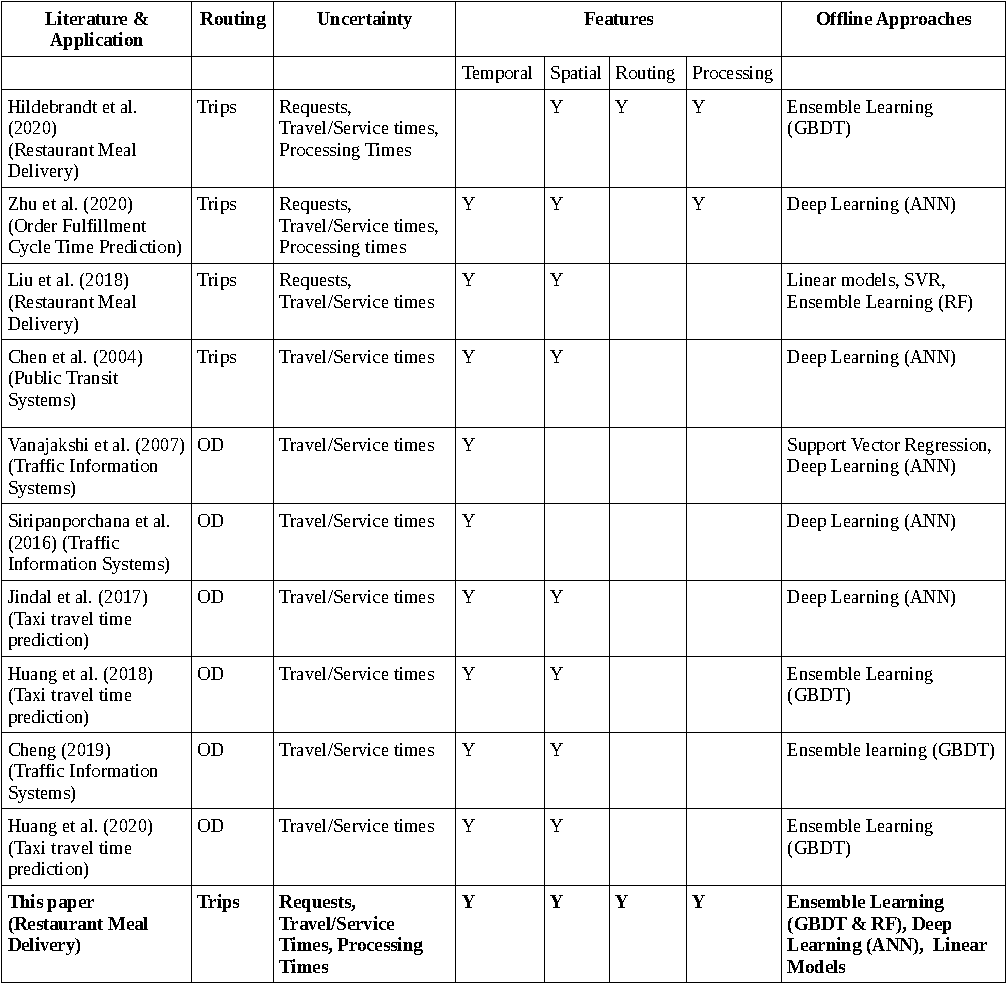
\includegraphics[width=\linewidth]{figures/LiteratureClassificationTable.pdf}
	\caption{Classification of Literature on Arrival Time Estimations with Supervised Learning}
	\label{fig:literatureTable}
\end{figure}
With \textit{Route type}, the table distinguishes arrival time estimation research that has been applied to vehicle route sequences consisting of single origin-destination (OD) pairs (referred to as \textit{OD} in the table) from those that have been applied to route sequences consisting of multiple OD pairs (referred to as \textit{trips} in the table) each.
By \textit{Uncertainty}, the table refers to uncertain elements in the underlying problem settings. Sources of Uncertainty considered here are requests, travel and service times, and processing times. Uncertainty in requests indicates that customer requests are not certainly known at the start of the problem and arrive dynamically over time. Uncertainty in travel and service times expresses itself through uncertain weather conditions, traffic congestion or individual challenges when serving customers (e.g. parking or waiting times). Uncertainty in processing occurs when two stochastic processes are synchronized (e.g. the synchronization of bus ride and bus boarding, or meal preparation and delivery). From the solution view, we classify the literature based on features and supervised learning algorithms used for travel time prediction. The \textit{features} column distinguishes between temporal, spatial, routing and processing features.
Temporal and spatial features include time and space related variables respectively. Examples for former are time stamps at a start/end point or historical travel times, and examples for latter are GPS coordinates or distances between locations. Processing and routing features give information about the uncertainty in processing times (e.g. meal preparation or bus boarding time) and the properties of a trip (e.g. number of stops in a trip) respectively.
The column \textit{Offline Approaches} presents all offline supervised learning approaches used in the respective literature, regardless of whether they were used as the primary approach to predict arrival times or solely for comparison purposes. 

A noticeable amount of research on arrival time prediction for vehicle trips via  supervised learning has been done in the field of bus arrival time prediction. \citet{Chen2004_ANNKalman} estimate arrival times for bus trips based on manually selected spatial, temporal, and routing information via neural networks. [Compare with related papers that estimate arrival times for bus trips].

Significant arrival time estimation research was also conducted for origin-destination problems in different subfields of intelligent transportation systems.

To predict travel times on freeways for different short-term forecasting horizons, \citet{Vanajakshi2007} use support vector regression (SVR) based on estimated route travel times from prior research and conclude that SVR performs comparably well to artificial neural networks (ANN).
\citet{Siripanpornchana2016_AnnWithDbnFS} propose a deep learning architecture consisting of a deep belief network and a sigmoid regression layer. Former learns features in an unsupervised fashion based on historical route travel times as inputs, latter then estimates travel times based on these learned features. \citet{Cheng2019_GBDT} make use of GBDTs using manually selected travel time features and traffic state related variables. They report that the ensemble learning approach with GBDTs outperforms feed-forward
neural networks and support vector machines.

For taxi travel time prediction, \citet{jindal2017unified} propose a unified approach based on raw NYC taxi data. They concatenate two neural networks, where the first one uses spatial features to predict travel distances, and the second one uses these predicted distances and additional temporal information to predict travel times. They solely compared their approach to other deep learning architectures.
In contrast to them, \citet{Huang2018_GBDT} and \citet{huang2020travel_GBDT} compare several tree-based learning methods to predict travel times on different horizons each based on NYC taxi data as well, among them random forests (both), GBDTs (both), and CART (only \citet{huang2020travel_GBDT}). While \citet{Huang2018_GBDT} selected features by means of principal component analysis, \citet{huang2020travel_GBDT} engineered them manually. Both ended up using spatial and temporal features mainly. Their results indicate that all tree-based ensemble methods are able to predict travel times more accurately than the respective benchmark algorithms (CART and naive approach in \citet{huang2020travel_GBDT}; linear and logistic regression in \citet{Huang2018_GBDT}).

\section{Summary}